\documentclass[aspectratio=169]{beamer}

% Theme moderne
\usetheme{Madrid}
\usecolortheme{seahorse}

% Packages
\usepackage[utf8]{inputenc}
\usepackage[T1]{fontenc}
\usepackage[french]{babel}
\usepackage{graphicx}
\usepackage{booktabs}
\usepackage{tikz}
\usetikzlibrary{positioning}
\usepackage{xcolor}

% Couleurs personnalisées
\definecolor{mainblue}{RGB}{41, 128, 185}
\definecolor{accentorange}{RGB}{230, 126, 34}
\definecolor{darkgray}{RGB}{52, 73, 94}
\definecolor{lightgray}{RGB}{236, 240, 241}

\setbeamercolor{structure}{fg=mainblue}
\setbeamercolor{frametitle}{bg=mainblue,fg=white}
\setbeamercolor{title}{bg=mainblue,fg=white}

% Informations
\title{Évaluation Comparative de Modèles d'Apprentissage Automatique}
\subtitle{Détection d'Intrusions Réseau : Modèles Tabulaires vs Graph Neural Networks}
\author{Cedric Tanekeu}
\institute{Projet de Synthèse}
\date{Automne 2025}

\begin{document}

% ============ PAGE DE TITRE ============
\begin{frame}
\titlepage
\end{frame}

% ============ TABLE DES MATIÈRES ============
\begin{frame}{Plan de la présentation}
\tableofcontents
\end{frame}

% ============ SECTION 1 : INTRODUCTION ============
\section{Introduction \& Contexte}

\begin{frame}{Contexte : La Cybersécurité}
\begin{columns}[T]
\column{0.5\textwidth}
\textbf{Problématique}
\begin{itemize}
    \item Cyberattaques de plus en plus sophistiquées
    \item IDS traditionnels (signatures) limités
    \item Nécessité de détecter les nouvelles menaces
\end{itemize}

\vspace{0.5cm}
\textbf{Défis}
\begin{itemize}
    \item Classes déséquilibrées (80\% trafic normal)
    \item Attaques rares difficiles à détecter
    \item Généralisation sur nouvelles attaques
\end{itemize}

\column{0.5\textwidth}
\begin{block}{Notre Approche}
Comparer deux paradigmes :
\begin{enumerate}
    \item \textcolor{darkgray}{Modèles tabulaires classiques}
    \item \textcolor{accentorange}{\textbf{Graph Neural Networks (GNN)}}
\end{enumerate}
\end{block}

\vspace{0.3cm}
\begin{alertblock}{Question de recherche}
Les GNN apportent-ils une amélioration significative par rapport aux modèles classiques ?
\end{alertblock}
\end{columns}
\end{frame}

\begin{frame}{Objectifs de l'étude}
\begin{enumerate}
    \item Établir des \textbf{références solides} avec modèles classiques sur CSE-CIC-IDS2018
    
    \item Identifier les \textbf{limitations} des approches tabulaires
    
    \item Construire un \textbf{graphe de similarité} (k-NN) entre flux réseau
    
    \item Évaluer \textbf{4 architectures GNN} : GCN, GAT, GraphSAGE, GAE
    
    \item Comparer de manière \textbf{objective} : mêmes données, mêmes métriques
\end{enumerate}
\end{frame}

% ============ SECTION 2 : DONNÉES ============
\section{Dataset \& Méthodologie}

\begin{frame}{Dataset : CSE-CIC-IDS2018}
\begin{columns}[T]
\column{0.6\textwidth}
\textbf{Caractéristiques}
\begin{itemize}
    \item Dataset moderne (2018)
    \item Trafic réel capturé en environnement universitaire
    \item \textcolor{accentorange}{\textbf{3 millions de flux}} pour notre étude
    \item 78-80 features (statistiques réseau)
    \item 10 classes retenues
\end{itemize}

\vspace{0.3cm}
\textbf{Types d'attaques}
\begin{itemize}
    \item DDoS (HOIC, LOIC)
    \item DoS (Hulk, SlowHTTPTest, Slowloris, GoldenEye)
    \item Brute Force (FTP, SSH)
    \item Bot, Infiltration
\end{itemize}

\column{0.4\textwidth}
\begin{block}{Déséquilibre}
\begin{itemize}
    \item Train : 80\% Benign
    \item Test : 72\% Benign
    \item Classes rares : $<$ 0.1\%
\end{itemize}
\end{block}

\vspace{0.3cm}
\begin{exampleblock}{Challenge}
Détecter les classes ultra-minoritaires tout en maintenant de bonnes performances globales
\end{exampleblock}
\end{columns}
\end{frame}

\begin{frame}{Pipeline de prétraitement}
\begin{center}
\begin{tikzpicture}[node distance=1.5cm, auto]
    \node[draw, rectangle, fill=lightgray, minimum width=2.5cm, minimum height=0.8cm, align=center] (raw) {Données brutes\\3M lignes};
    \node[draw, rectangle, fill=mainblue!20, minimum width=2.5cm, minimum height=0.8cm, right=of raw, align=center] (clean) {Nettoyage\\67 features};
    \node[draw, rectangle, fill=mainblue!40, minimum width=2.5cm, minimum height=0.8cm, right=of clean, align=center] (norm) {Normalisation\\StandardScaler};
    \node[draw, rectangle, fill=mainblue!60, minimum width=2.5cm, minimum height=0.8cm, right=of norm, align=center] (split) {Split 70/30\\Stratifié};

    \draw[->, thick] (raw) -- (clean);
    \draw[->, thick] (clean) -- (norm);
    \draw[->, thick] (norm) -- (split);
\end{tikzpicture}
\end{center}

\vspace{0.5cm}

\textbf{Étapes clés :}
\begin{itemize}
    \item Suppression colonnes : Timestamp, IP, Port (éviter target leakage)
    \item Gestion valeurs manquantes : 1.1M remplacées par médiane
    \item Suppression classes rares : moins de 100 échantillons
    \item Encodage labels : LabelEncoder (0-9)
\end{itemize}
\end{frame}

% ============ SECTION 3 : MODÈLES TABULAIRES ============
\section{Résultats : Modèles Tabulaires}

\begin{frame}{Modèles évalués (18 algorithmes)}
\begin{columns}[T]
\column{0.5\textwidth}
\textbf{Modèles linéaires}
\begin{itemize}
    \item Logistic Regression
    \item SGDClassifier
    \item LinearSVC
    \item Ridge Classifier
\end{itemize}

\vspace{0.3cm}
\textbf{Ensembles (Bagging)}
\begin{itemize}
    \item Random Forest
    \item Extra Trees
    \item Bagging Classifier
\end{itemize}

\column{0.5\textwidth}
\textbf{Ensembles (Boosting)}
\begin{itemize}
    \item \textcolor{accentorange}{\textbf{XGBoost}}
    \item LightGBM
    \item Gradient Boosting
    \item HistGradient Boosting
    \item AdaBoost
\end{itemize}

\vspace{0.3cm}
\textbf{Autres}
\begin{itemize}
    \item Decision Tree
    \item k-NN
    \item Naive Bayes (Gaussian, Bernoulli)
\end{itemize}
\end{columns}
\end{frame}

\begin{frame}{Résultats : Performances}
\begin{center}
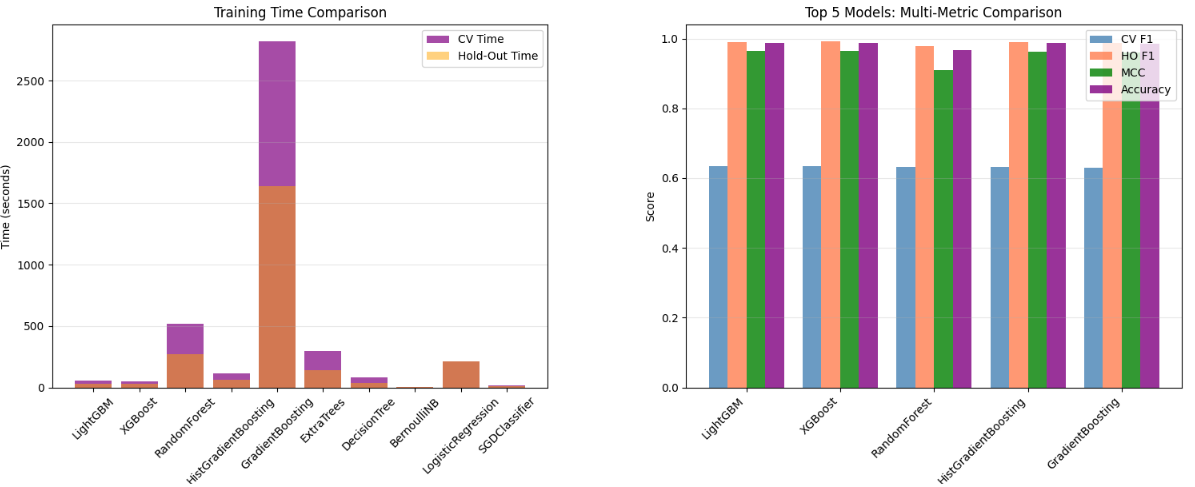
\includegraphics[width=0.9\textwidth]{../figures/Screenshot1.png}
\end{center}

\textbf{Observations clés :}
\begin{itemize}
    \item Modèles d'ensemble : meilleurs F1-scores (0.6-0.9)
    \item \textcolor{red}{Accuracy élevée mais trompeuse} (90-100\%)
    \item Cohérence entre CV et Hold-out
\end{itemize}
\end{frame}

\begin{frame}{Résultats : Temps \& Multi-métriques}
\begin{center}
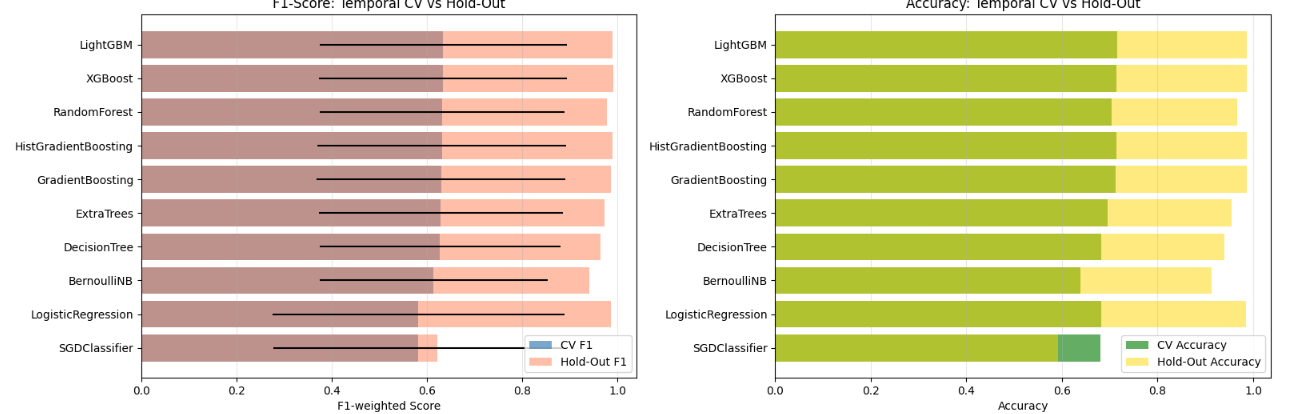
\includegraphics[width=0.9\textwidth]{../figures/Screenshot2.png}
\end{center}

\textbf{Constat :}
\begin{itemize}
    \item HistGradientBoosting : très lent (45 min)
    \item Accuracy $\sim$95-100\% vs F1-score $\sim$60-65\%
    \item \textcolor{red}{\textbf{Divergence révélatrice du déséquilibre}}
\end{itemize}
\end{frame}

\begin{frame}{Meilleur modèle tabulaire : XGBoost}
\begin{block}{Performances XGBoost}
\begin{itemize}
    \item Accuracy : \textbf{91.5\%}
    \item F1-weighted : \textbf{87.4\%}
    \item \textcolor{red}{F1-macro : 23.9\%} ← Problème !
    \item \textcolor{red}{Balanced Accuracy : 33.3\%}
    \item \textcolor{red}{MCC : $\approx$ 0}
\end{itemize}
\end{block}

\vspace{0.3cm}

\begin{alertblock}{Problème majeur}
\textbf{Biais vers la classe majoritaire "Benign"}
\begin{itemize}
    \item Excellentes performances sur attaques volumétriques (DDoS)
    \item Moyennes sur attaques lentes (Slowloris)
    \item \textcolor{red}{\textbf{Nulles sur classes nouvelles (Bot, Infiltration)}}
\end{itemize}
\end{alertblock}
\end{frame}

% ============ SECTION 4 : GRAPH NEURAL NETWORKS ============
\section{Approches Graphes (GNN)}

\begin{frame}{Construction du graphe k-NN}
\textbf{Motivation :} Exploiter la \textcolor{accentorange}{\textbf{structure de similarité}} entre flux réseau

\vspace{0.5cm}

\begin{columns}[T]
\column{0.5\textwidth}
\textbf{Méthodologie}
\begin{itemize}
    \item 100,000 nœuds (flux réseau)
    \item 67 features par nœud
    \item k-NN avec k=10
    \item Distance euclidienne
\end{itemize}

\vspace{0.3cm}
\textbf{Résultat}
\begin{itemize}
    \item 484,602 arêtes
    \item Degré moyen : 9.69
    \item 3,186 composantes
    \item Plus grande : 68,241 nœuds
\end{itemize}

\column{0.5\textwidth}
\begin{exampleblock}{Principe}
Un flux similaire à des flux d'attaque a plus de chances d'être malveillant
\end{exampleblock}

\vspace{0.3cm}
\begin{block}{Avantage}
Les classes rares "empruntent" des informations de leurs voisins
\end{block}
\end{columns}
\end{frame}

\begin{frame}{Architectures GNN testées}
\begin{enumerate}
    \item \textbf{GCN} (Graph Convolutional Network)
    \begin{itemize}
        \item Agrège uniformément les voisins
        \item Simple et efficace
    \end{itemize}
    
    \item \textbf{GAT} (Graph Attention Network)
    \begin{itemize}
        \item Mécanisme d'attention
        \item Pondère dynamiquement les voisins
    \end{itemize}
    
    \item \textbf{\textcolor{accentorange}{GraphSAGE}} (Sample and Aggregate)
    \begin{itemize}
        \item Échantillonnage de voisins
        \item \textcolor{accentorange}{\textbf{Apprentissage inductif}}
        \item Crucial pour flux temps-réel
    \end{itemize}
    
    \item \textbf{GAE} (Graph Auto-Encoder)
    \begin{itemize}
        \item Apprentissage non supervisé
        \item Reconstruction de structure
    \end{itemize}
\end{enumerate}
\end{frame}

\begin{frame}{Résultats GNN : Mode Transductif}
\textbf{Mode transductif :} Le modèle connaît la structure complète du graphe

\vspace{0.5cm}

\begin{center}
\begin{tabular}{lccc}
\toprule
\textbf{Modèle} & \textbf{Accuracy} & \textbf{F1-macro} & \textbf{MCC} \\
\midrule
\textcolor{accentorange}{\textbf{GraphSAGE}} & \textbf{98.91\%} & \textbf{90.27\%} & \textbf{0.9659} \\
GCN & 98.75\% & 88.76\% & -- \\
GAT & 94.83\% & 77.98\% & -- \\
\midrule
\textcolor{gray}{XGBoost (réf.)} & \textcolor{gray}{91.5\%} & \textcolor{gray}{23.9\%} & \textcolor{gray}{$\approx$ 0} \\
\bottomrule
\end{tabular}
\end{center}

\vspace{0.5cm}

\begin{block}{Performance exceptionnelle de GraphSAGE}
\textcolor{accentorange}{\textbf{+66.4 points}} de F1-macro par rapport à XGBoost !
\end{block}
\end{frame}

\begin{frame}{Résultats GNN : Mode Inductif}
\textbf{Mode inductif :} Généralisation sur flux \textcolor{accentorange}{\textbf{jamais vus}}

\vspace{0.5cm}

\begin{center}
\begin{tabular}{lccc}
\toprule
\textbf{Modèle} & \textbf{Accuracy} & \textbf{F1-macro} & \textbf{MCC} \\
\midrule
\textcolor{accentorange}{\textbf{GraphSAGE}} & \textbf{98.87\%} & \textbf{79.85\%} & \textbf{0.9649} \\
GCN & 98.77\% & 88.02\% & -- \\
GAT & 95.01\% & 72.19\% & -- \\
\bottomrule
\end{tabular}
\end{center}

\vspace{0.5cm}

\begin{exampleblock}{Robustesse remarquable}
Dégradation modérée : 90.27\% → 79.85\% (\textcolor{accentorange}{\textbf{−10 points}})
\end{exampleblock}

\vspace{0.3cm}

\textbf{Crucial pour IDS temps-réel} où nouveaux flux apparaissent constamment
\end{frame}

\begin{frame}{Pourquoi les GNN réussissent-ils ?}
\textbf{3 mécanismes clés :}

\vspace{0.5cm}

\begin{enumerate}
    \item \textbf{Propagation d'information}
    \begin{itemize}
        \item Flux rares (3 exemples) connectés à flux similaires
        \item "Emprunt" de connaissances des voisins
        \item \textcolor{accentorange}{\textbf{Résultat : 100\% détection DDOS LOIC-UDP}}
    \end{itemize}
    
    \vspace{0.3cm}
    
    \item \textbf{Lissage des représentations}
    \begin{itemize}
        \item Features bruitées moyennées avec voisins k-NN
        \item Représentation plus robuste
    \end{itemize}
    
    \vspace{0.3cm}
    
    \item \textbf{Contexte relationnel}
    \begin{itemize}
        \item Modèles tabulaires : chaque flux indépendant
        \item GNN : un flux suspect entouré d'autres flux suspects = plus probable d'être une attaque
    \end{itemize}
\end{enumerate}
\end{frame}

% ============ SECTION 5 : COMPARAISON ============
\section{Comparaison \& Analyse}

\begin{frame}{XGBoost vs GraphSAGE : Le choc des titans}
\begin{center}
\begin{tabular}{lcc}
\toprule
\textbf{Métrique} & \textbf{XGBoost} & \textbf{GraphSAGE} \\
\midrule
Accuracy & 91.5\% & \textcolor{accentorange}{\textbf{98.91\%}} \textcolor{darkgray}{(+7.4)} \\
F1-weighted & 87.4\% & \textcolor{accentorange}{\textbf{98.87\%}} \textcolor{darkgray}{(+11.4)} \\
\textbf{F1-macro} & \textcolor{red}{23.9\%} & \textcolor{accentorange}{\textbf{90.27\%}} \textcolor{accentorange}{\textbf{(+66.4)}} \\
\textbf{Balanced Acc.} & \textcolor{red}{33.3\%} & \textcolor{accentorange}{\textbf{88.29\%}} \textcolor{accentorange}{\textbf{(+55)}} \\
\textbf{MCC} & \textcolor{red}{$\approx$ 0} & \textcolor{accentorange}{\textbf{0.9659}} \\
\bottomrule
\end{tabular}
\end{center}

\vspace{0.5cm}

\begin{block}{Différence spectaculaire}
GraphSAGE résout le problème du \textcolor{red}{\textbf{biais vers la classe majoritaire}}
\end{block}

\vspace{0.3cm}

\textbf{Classes ultra-minoritaires :}
\begin{itemize}
    \item DDOS LOIC-UDP (3 ex.) : \textcolor{accentorange}{\textbf{100\%}} détection
    \item Classes volumétriques : F1 $\approx$ 0.99-1.00
    \item Classes rares : F1 $\approx$ 0.75-0.92
\end{itemize}
\end{frame}

\begin{frame}{Quand privilégier quelle approche ?}
\begin{columns}[T]
\column{0.5\textwidth}
\begin{block}{Modèles Tabulaires}
\textbf{Avantages}
\begin{itemize}
    \item Implémentation simple
    \item Rapides (sauf HistGB)
    \item Interprétables (SHAP)
    \item Bien connus des équipes
\end{itemize}

\vspace{0.3cm}
\textbf{Utiliser quand :}
\begin{itemize}
    \item Attaques courantes
    \item Classes bien représentées
    \item Besoin d'explicabilité
    \item Ressources limitées
\end{itemize}
\end{block}

\column{0.5\textwidth}
\begin{block}{Graph Neural Networks}
\textbf{Avantages}
\begin{itemize}
    \item \textcolor{accentorange}{\textbf{Excellents sur classes rares}}
    \item Généralisation inductif
    \item Exploitation structure
    \item MCC élevé
\end{itemize}

\vspace{0.3cm}
\textbf{Utiliser quand :}
\begin{itemize}
    \item Classes rares critiques
    \item Nouvelles attaques
    \item Vision contextuelle
    \item Few-shot learning
    \item Ressources GPU disponibles
\end{itemize}
\end{block}
\end{columns}

\vspace{0.5cm}
\centering
\textbf{\textcolor{accentorange}{Architecture hybride recommandée : GNN + Tabulaire}}
\end{frame}

\begin{frame}{Limitations de l'étude}
\begin{columns}[T]
\column{0.5\textwidth}
\textbf{Méthodologiques}
\begin{itemize}
    \item Un seul dataset principal
    \item Sous-échantillonnage (3M)
    \item Graphe limité (100k nœuds)
    \item Ressources GPU limitées
\end{itemize}

\vspace{0.3cm}
\textbf{Techniques}
\begin{itemize}
    \item Conflits dépendances Python
    \item Temps entraînement longs
    \item Construction graphe k-NN coûteuse
\end{itemize}

\column{0.5\textwidth}
\textbf{Contextuelles}
\begin{itemize}
    \item Environnement universitaire
    \item Focus DDoS/DoS
    \item Trafic chiffré non traité
    \item Graphe statique (non temporel)
\end{itemize}

\vspace{0.3cm}
\textbf{GNN}
\begin{itemize}
    \item Interprétabilité limitée
    \item Scalabilité (millions nœuds)
    \item Sensibilité construction graphe
\end{itemize}
\end{columns}
\end{frame}

% ============ SECTION 6 : CONCLUSION ============
\section{Conclusion \& Perspectives}

\begin{frame}{Conclusions principales}
\begin{enumerate}
    \item \textbf{Modèles tabulaires atteignent leurs limites}
    \begin{itemize}
        \item Accuracy élevée mais \textcolor{red}{\textbf{trompeuse}}
        \item F1-macro faible révèle biais vers classe majoritaire
        \item Échouent sur classes rares et nouvelles attaques
    \end{itemize}
    
    \vspace{0.3cm}
    
    \item \textbf{GNN apportent amélioration spectaculaire}
    \begin{itemize}
        \item \textcolor{accentorange}{\textbf{GraphSAGE : +66 points de F1-macro}}
        \item 100\% détection classes ultra-minoritaires
        \item Robuste en mode inductif
    \end{itemize}
    
    \vspace{0.3cm}
    
    \item \textbf{Le graphe k-NN est la clé}
    \begin{itemize}
        \item Capture similarité entre flux
        \item Propagation d'information
        \item Contexte relationnel
    \end{itemize}
\end{enumerate}
\end{frame}

\begin{frame}{Perspectives de recherche}
\textbf{Court terme}
\begin{itemize}
    \item Graphes temporels (snapshots horaires)
    \item Graphes IP-IP (au lieu de k-NN)
    \item Architectures GNN avancées
\end{itemize}

\vspace{0.3cm}

\textbf{Moyen terme}
\begin{itemize}
    \item Autres datasets (CIC-DDoS2019, Bot-IoT)
    \item Semi-supervisé / Few-shot learning
    \item Robustesse aux attaques adversariales
\end{itemize}

\vspace{0.3cm}

\textbf{Long terme}
\begin{itemize}
    \item Federated Learning avec GNN
    \item Explicabilité GNN pour analystes SOC
    \item Système hybride temps-réel
\end{itemize}
\end{frame}

\begin{frame}{Contributions}
\begin{block}{Contributions scientifiques}
\begin{enumerate}
    \item Pipeline reproductible pour CSE-CIC-IDS2018
    \item Première comparaison systématique tabulaire vs GNN
    \item Résultats quantitatifs clairs sur classes rares
    \item Analyse détaillée des cas d'usage
\end{enumerate}
\end{block}

\vspace{0.3cm}

\begin{exampleblock}{Impact pratique}
\textbf{Recommandation :} Architecture hybride
\begin{itemize}
    \item Modèles tabulaires : première ligne de défense
    \item GNN : scénarios critiques (classes rares, nouvelles attaques)
\end{itemize}
\end{exampleblock}
\end{frame}

% ============ MERCI ============
\begin{frame}[plain]
\begin{center}
\vspace{2cm}
{\Huge \textcolor{mainblue}{\textbf{Merci de votre attention}}}

\vspace{1cm}

{\Large Questions ?}

\vspace{1.5cm}

\textcolor{darkgray}{Cedric Tanekeu}

\textcolor{darkgray}{Projet de Synthèse -- Automne 2025}
\end{center}
\end{frame}

% ============ BACKUP SLIDES ============
\appendix

\begin{frame}{Backup : Détails techniques}
\textbf{Configuration GNN}
\begin{itemize}
    \item 2 couches
    \item Hidden dimension : 64
    \item Dropout : 0.5-0.6
    \item Optimiseur : Adam (lr=0.01)
    \item Early stopping : patience 30
\end{itemize}

\vspace{0.3cm}

\textbf{Environnement}
\begin{itemize}
    \item Google Colab (CPU/GPU T4, 51 GO RAM)
    \item Python 3.12
    \item PyTorch 2.0.1, PyTorch Geometric
    \item Scikit-learn, XGBoost, LightGBM
\end{itemize}
\end{frame}

\end{document}

